\chapter{Algorithm Description} \label{chap:algorithm}

Originally, our problem statement required the analysis of interactions between three types of traffic (pedestrians, bicycles, and cars). With this in mind, a free-agent simulation was designed with three corresponding sub-classes of agent. Agents were given the ability to read color data from image files, and respond if certain colors were encountered. After being spawned, agents would use this method to find their way towards a goal across a ‘map’ image (such as Figure \ref{fig:map-roundabout}). This navigation was accomplished through a system of vector calculations: a force vector pulled each agent towards its goal, while proximity to other agents and dangerous areas in their surroundings compounded to produce a final direction. We intended to run several iterations of these simulations, and examine results and emergent behaviour. As will be discussed, this presented numerous issues in maps more complex than straight lanes, and was ultimately abandoned for a more implementable method.

\begin{figure}[h]
    \centering
    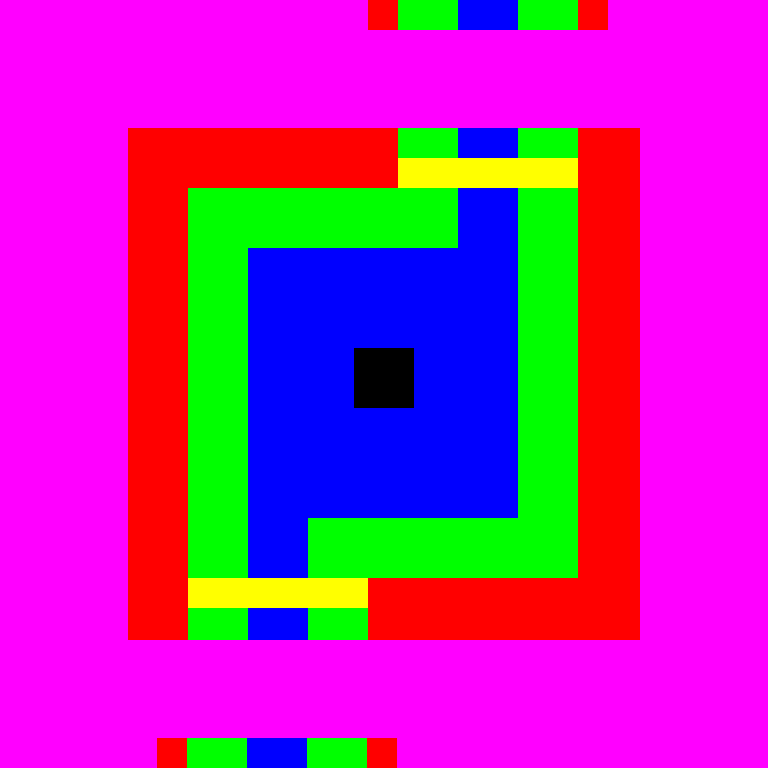
\includegraphics[width=3in]{images/map-roundabout.png}
    \caption{A handmade map of a roundabout with sidewalks, bike lanes, crosswalks, and two exit lanes.}
    \label{fig:map-roundabout}
\end{figure}

The current iteration simplifies certain aspects to create a more reliable and usable program. Rather than image files, maps are encoded as patterns of characters stored in \texttt{.dzone} (text) files. Although not as straightforward to visualise, this aids in the creation of maps and in the extraction of information from them. Additionally, the size of each map has been significantly reduced; in the free agents model, maps were 512x512 pixel squares, and color information was collected from a radius around each agent. In the current version, maps are represented in a 16x16 grid (excluding outer spawn areas), such that each character acts as a distinct ‘tile’ rather than a piece of an area. This brings the simulation away from the idea freely moving agents, and closer to a cellular automata approach.

The agents are not, however, entirely autonomous. They have been given intelligence and determination in the form of a Python implementation of the popular A* pathfinding algorithm. At each tick, pedestrians evaluate their surroundings (including how “dangerous” each tile near them is) and plan a route to their goal. If the pathfinding algorithm cannot find a path to the target, a best-effort choice is made to the neighbour that brings the agent closest to the target.

To reduce the complexity of the simulation, we decided that the implementation of a bicycle agent type should be postponed. As the interaction between cars and pedestrians presents a sufficiently complex simulation challenge, it was prioritised, with the bicycle simulation being an area of future work.
When a simulation is run, both pedestrians and cars are spawned at designated locations. As they advance onto the map, more appear at a specified (and adjustable) rate.

There are three different types of tile -- sidewalk, street, and crosswalk (where a crosswalk represents what is considered the `shared space'). Streets and crosswalks are further divided by the direction in which car agents should be moving over them, in order for us to be able to create specific lanes for them to travel along (instead of also having them use the pathfinding method). This further simplification was done because in reality cars entirely follow lanes, and would never purposefully drive into oncoming traffic or across pavement in any circumstances.

When a pedestrian is spawned, it is randomly assigned to have one of the other pedestrian spawn points as its goal. It formulates a set of tiles it will move through to reach that goal, then advances one tile along this path. The path is stored and recomputed at each tick in order to avoid collisions. When routes are being considered, street tiles are seen as much more `dangerous' than either sidewalk or crosswalk. This translates into pedestrians always choosing to avoid the street, and to greatly prefer to use crosswalks than to jaywalk.

Car agents, on the other hand, process crosswalk tiles exactly the same as other street tiles. However, car agents will not advance if they detect a pedestrian within two tiles directly in front of them. This means a car will never drive directly into a pedestrian, even if they are crossing a shared space.

As the simulation runs, variables are incremented to count the number of cars and pedestrians that reach their respective goals. The number of failed spawns, or the number of agents that could not be created due to their spawn fields being occupied by other agents, is also recorded in order to measure how crowded the simulation has become. This data can then be collected in CSV format and used as measure of the efficiency of each simulation. Each simulation run is also saved as a trace, in JSON format, to allow for later playback.
